\documentclass[]{article}

% Import packages
\usepackage[fleqn]{amsmath}
\usepackage{graphicx}
\usepackage[export]{adjustbox}
\usepackage{xcolor}
\usepackage{adjustbox}
\usepackage{array}

% Page initialization
\setlength{\topmargin}{-.3 in}
\setlength{\oddsidemargin}{0in}
\setlength{\evensidemargin}{0in}
\setlength{\textheight}{9.in}
\setlength{\textwidth}{6.5in}
\pagestyle{empty}

%==============================================================%
%------------------------START-DOCUMENT------------------------%
%==============================================================%
\begin{document}

%----------------------------HEADER----------------------------%

\begin{center}
    {\Large AERO 422 Homework \#3}\\ % Homework number
    \vspace{0.2 cm}
    Instructor: Vedang Deshpande\\ % Instructor name
    \vspace{0.2 cm}
    Due: October 05, 2021 at 12:00a.m.\\ % Due date
    \vspace{0.2 cm}
    Fall 2021\\ % semester
    \vspace{0.2 cm}
    (\textbf{28 Points})\\
\end{center}

\vspace{0.2 cm}

\begin{enumerate}

    %---------------------------PROBLEM-1--------------------------%
    \item A block diagram for a spacecraft docking control problem is given by
    % insert image
    \begin{figure}[h]
        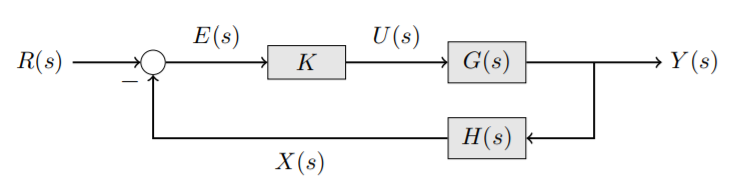
\includegraphics[scale=0.8,center]{AERO_422_HW3_P1.png}
    \end{figure}
    \\where $K$ represents the controller. It is important to keep in mind that this is a docking problem, so overshooting (going past) the reference input is not desired.

    \begin{enumerate}
        \item (\textbf{1 point}) Evaluate the transfer function from $U(s)$ to $Y(s)$ if the input/output relationship satisfies
        $$m\ddot{y}(t) + c\dot{y}(t) = u(t)$$
        \textcolor{blue}{
        Solution in other document.
        }

        \item (\textbf{1 point}) Evaluate the transfer function from $Y(s)$ to $X(s)$ if
        $$\dot{x}(t) + \tau x(t) = \tau y(t)$$
        \textcolor{blue}{
        Solution in other document.
        }

        \item (\textbf{2 points}) Consider the closed loop transfer function $T(s)$, such that $Y(s) = T(s) \cdot R(s)$. $T(s)$ has the form, 
        $$T(s) = \frac{a_1s + 60}{b_3s^3 + b_2s^2 + b_1s + 60}$$        
        Determine the values of $a_1$, $b_3$, $b_2$, $b_1$ is the text boxes below when
        $K = 5$, $m = 2$, $c = 7$, and $\tau = 12$.\\
        \textcolor{blue}{
        Solution in other document.
        }

        \item (\textbf{12 points}) Consider three cases of parameter values:\\\\
        Case 1: $K = 30$, $m = 2$, $c = 7$, $\tau = 0.2$\\
        Case 2: $K = 5$, $m = 2$, $c = 7$, $\tau = 12$\\
        Case 3: $K = 10$, $m = 2$, $c = 7$, $\tau = 0.1$\\\\
        For all cases,\\\\
        i.) Plot $y(t)$ if $r(t) = 1(t), t \geq 0$. You may use the "step" command in MATLAB.\\\\
        ii.) Plot the pole-zero map of $T(s)$ using MATLAB.\\\\
        iii.) For each case, determine whether or not the system is stable.\\\\
        iv.) For each case, determine whether or not this parameter set is acceptable for the problem application we have considered.\\
        \textcolor{blue}{
        Substitute the parameters from Case 1 into the general form of the transfer function. Using the MATLAB tools "step" and "pzmap" yield the follwoing results:\\
         % insert image of Case 1
        \begin{figure}[h]
            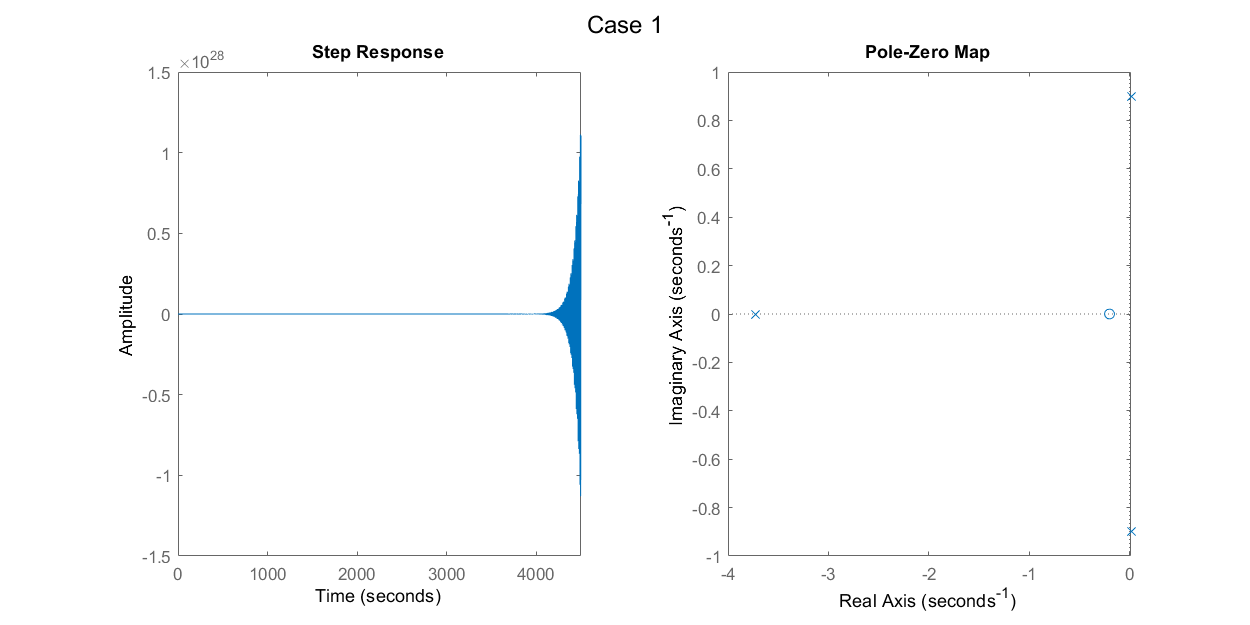
\includegraphics[scale=0.45,center]{AERO_422_HW3_P1case1.png}
        \end{figure}\\
        From the figure above, we can see that this closed-loop system diverges and thus, is unstable. We can also infer this from observing the poles of the system since two of them are (slightly) positive.\\\\
        This set of parameters is not acceptable for our problem application. Divergent oscillations are not a desired output for a spacecraft docking system.\\\\
        Substitute the parameters from Case 2 into the general form of the transfer function. Using the MATLAB tools "step" and "pzmap" yield the follwoing results:\\
         % insert image of Case 2
        \begin{figure}[h]
            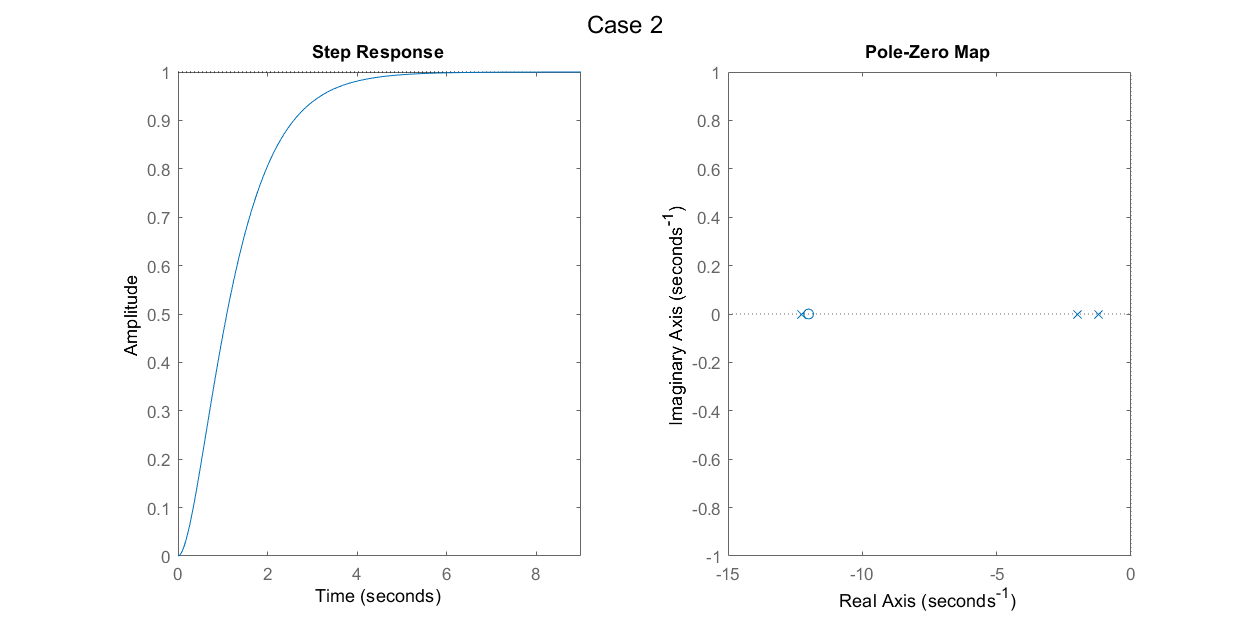
\includegraphics[scale=0.45,center]{AERO_422_HW3_P1case2.png}
        \end{figure}\\
        From the figure above, we can see that this closed-loop system approaches a steady state value without oscillations. We can also infer this from observing the poles of the system since they are all have negative real components and no imaginary components.\\\\
        This set of parameters is acceptable for our problem application. We want a spacecraft docking system to approach the target attitude and position without overshooting or oscillating.\\\\
        Substitute the parameters from Case 3 into the general form of the transfer function. Using the MATLAB tools "step" and "pzmap" yield the follwoing results:\\
         % insert image of Case 3
        \begin{figure}[h]
            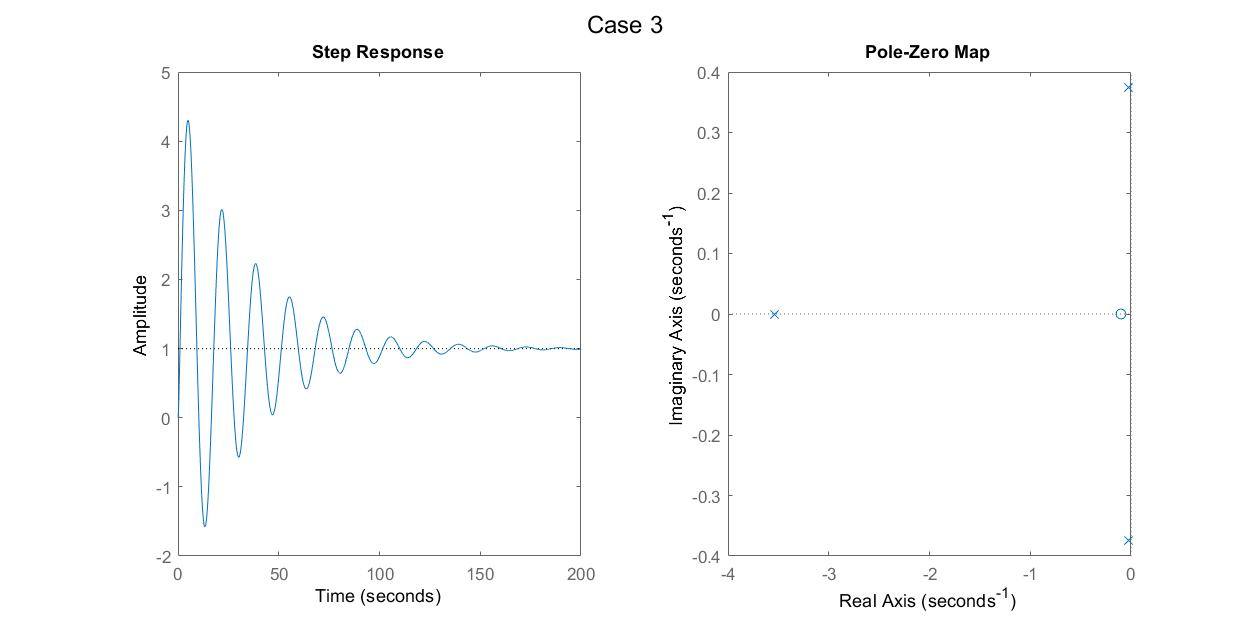
\includegraphics[scale=0.45,center]{AERO_422_HW3_P1case3.png}
        \end{figure}\\
        From the figure above, we can see that this closed-loop system converges and thus, is stable. We can also infer this from observing the poles of the system since they all have negative real components and two have non-zero imaginary components.\\\\
        Despite this system being stable, this set of parameters is not acceptable for our problem application. This is because we do not want erratic oscillations at any point during a docking procedure.\\\\
        \textbf{Note: a more in-depth solution to this problem is available in the other document. Additionally, the MATLAB code to produce the plots above is provided at the end of this document.}
        \vspace{0.3cm}
        }
    \end{enumerate}

    \item One of the poles for a transfer function was found to be $a+bj$. Below are the possible mode shapes corresponding to this pole. (Horizontal axis denotes time, and vertical axis denotes impulse response associated with the pole.) Describe the properties of the real and imaginary parts of the pole associated to each of the following mode shapes.
    
    \begin{enumerate}
        \item (\textbf{1 point}) % insert image of part a
        \adjustbox{valign=t}{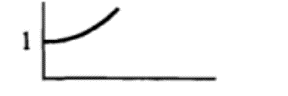
\includegraphics[scale=0.70,center]{AERO_422_HW3_P2a.png}}
        \textcolor{blue}{
        The impulse response of this system is diverging and without oscillations. Therefore, the pole of this transfer function has a positive real part and no imaginary part.\\
        $$a > 0,b = 0$$
        }

        \item (\textbf{1 point}) % insert image of part b
        \adjustbox{valign=t}{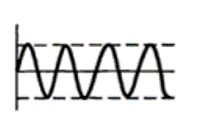
\includegraphics[scale=0.70,center]{AERO_422_HW3_P2b.png}}
        \textcolor{blue}{
        The impulse response of this system is purely oscillatory about a stable point. Therefore, the pole of this transfer function has no real part and and a non-zero imaginary part.\\
        $$a = 0,b \neq 0$$
        }

        \item (\textbf{1 point}) % insert image of part c
        \adjustbox{valign=t}{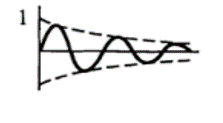
\includegraphics[scale=0.70,center]{AERO_422_HW3_P2c.png}}
        \textcolor{blue}{
        The impulse response of this system converges to a steady state value while oscillating. Therefore, the pole of this transfer function has a negative real part and and a non-zero imaginary part.\\
        $$a < 0,b \neq 0$$
        }

        \item (\textbf{1 point}) % insert image of part d
        \adjustbox{valign=t}{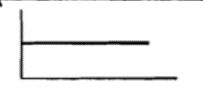
\includegraphics[scale=0.70,center]{AERO_422_HW3_P2d.png}}
        \textcolor{blue}{
        The impulse response of this system is completely stable. It does not diverge, or contain oscillations. Therefore, the pole of this transfer function is zero, both is real and imaginary parts.\\
        $$a = 0,b = 0$$
        }
    \end{enumerate}

    \item (\textbf{5 points}) Given a second order system with transfer function
    $$H(s) = \frac{s + 1}{2s^2 + 2s + 18}$$
    determine the natural frequency, damping ratio, rise time, percent overshoot, and settling time associated with the step response of this system.\\\\
    Hint: Note that the transfer function $H(s)$ is not in standard form. First manipulate $H(s)$ such that the denominator of $H(s)$ is comparable to the standard form. In practice, we ignore the zeros (i.e. numerator) of the transfer function, and calculate natural frequency and damping ratio by comparing the denominators.\\
    \textcolor{blue}{
    The first step is to evaluate the step response of the system. In Laplace-domain, this is equivalent the the multiplication of the transfer function and the step input.
    \begin{flalign*}
        Y(s) &= H(s) \cdot U(s)\\[5pt]
        &= \frac{s + 1}{2s^2 + 2s + 18} \cdot \frac{1}{s}\\
    \end{flalign*}
    Recall that the standard form of a second-order system is the following:
    \begin{flalign*}
        H_1(s) = \frac{\omega_n^2}{s^2 + 2 \zeta \omega_n s + \omega_n^2}
    \end{flalign*}
    We can redefine the step response as the convolution of two new functions, $H_1(s)$ and $H_2(s)$, where we assume that $H_1$ is the standard form of the second-order transfer function of this system.
    \begin{flalign*}
        H(s) &= \frac{s + 1}{s(2s^2 + 2s + 18)}\\[5pt]
        &= \frac{9}{s^2 + s + 9} \cdot \frac{s+1}{18}\\[5pt]
        &= H_1(s) \cdot H_2(s)
    \end{flalign*}
    From $H_1(s)$, we can directly compute the natural frequency and damping ratio.
    \begin{flalign*}
        \omega_n^2 = 9\\[5pt]
        \omega_n = 3\\\\
        2 \zeta \omega_n = 1\\[5pt]
        \zeta = \frac{1}{6}
    \end{flalign*}
    From natural frequency, we can approximate the rise time.
    \begin{flalign*}
        t_r &= \frac{1.8}{\omega_n}\\[5pt]
        &= \frac{1.8}{3}\\[5pt]
        &= 0.6
    \end{flalign*}
    From damping ratio, we can approximate the percent overshoot.
    \begin{flalign*}
        M_p &= e^{-\pi \zeta / \sqrt{1 - \zeta^2}}\\[5pt]
        &= e^{-\pi / \left(6 \sqrt{1 - (\frac{1}{6})^2}\right)}\\[5pt]
        &\approx 0.588\\[5pt]
        &= 58.8\%
    \end{flalign*}
    Lastly, we can calculate the settling time from the natural frequency and damping ratio.
    \begin{flalign*}
        t_s &= \frac{4.6}{\sigma} \text{, where } \sigma = \zeta \omega_n\\[5pt]
        t_s &= \frac{4.6}{\zeta \omega_n}\\[5pt]
        &= \frac{4.6}{3 \cdot (1/6)}\\[5pt]
        &= 9.2
    \end{flalign*}
    }
    \vspace{0.5cm}

    \item (\textbf{3 points}) Use Routh’s stability criterion to determine the range of controller gains $(K,K_I)$ such that closed loop system is stable.\\
    \begin{figure}[h]
        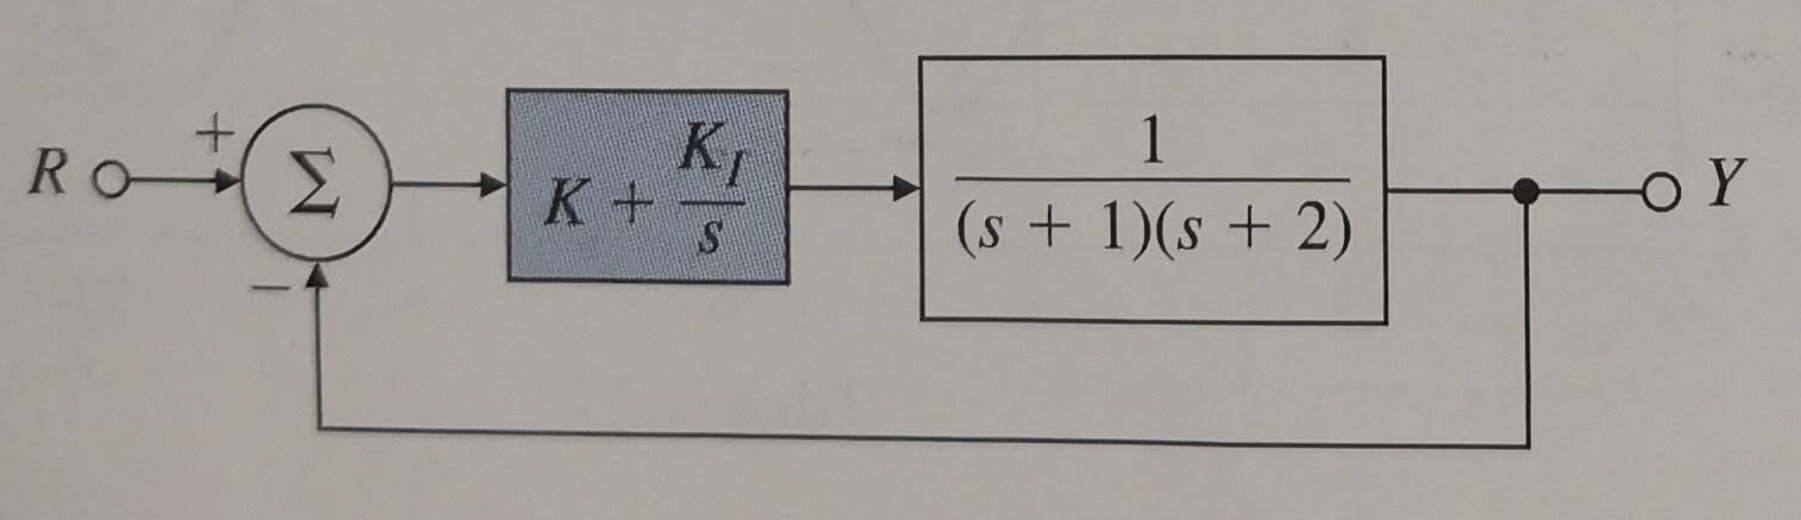
\includegraphics[scale=0.4,center]{AERO_422_HW3_P4.png}
    \end{figure}\\
    \textcolor{blue}{
    The closed-loop transfer function for this system is
    \begin{flalign*}
        T(s) &= \frac{Y(s)}{R(s)}\\[5pt]
        &= \frac{\left(K + \frac{K_I}{s}\right) \frac{1}{(s+1)(s+2)}}{1 + \left(K + \frac{K_I}{s}\right) \frac{1}{(s+1)(s+2)}}\\[5pt]
        &= \frac{Ks + K_I}{s^3 + 3s^2 + (2 + K)s + K_I}
    \end{flalign*}
    The characteristic equation for the clsoed-loop system is
    \begin{flalign*}
        1 + \left(K + \frac{K_I}{s}\right) \frac{1}{(s+1)(s+2)} = 0,
    \end{flalign*}
    which we may rewrite as
    \begin{flalign*}
        s^3 + 3s^2 + (2 + K)s + K_I = 0.
    \end{flalign*}
    The correspoinding Routh array is\\\\
    \begin{tabular}{ c|c c } 
        $s^3$ & $1$                & $2 + K$\\ 
        $s^2$ & $3$                & $K_I$  \\ 
        $s^1$ & $(6 + 3K - K_I)/3$ &        \\
        $s^0$ & $K_I$              &        \\
    \end{tabular}\\\\\\
    For internal stability, we must have
    \begin{flalign*}
        K_I > 0 \quad \text{and} \quad K > \frac{1}{3} K_I - 2
    \end{flalign*}
    }
\end{enumerate}

\end{document}